\section{Problem Formulation}
\subsection{Speckle problem}
Speckles capture the information of the spatial distribution of defects. However, the quasiparticle band structure information is embedded in the \ac{QPI} pattern of an individual defect. Therefore, to address the challenge of speckles is to disentangle the spatial information from the \ac{QPI} pattern, and this can be formulated mathematically as a deconvolution problem. 
\par \noindent Recall that we can write the modulation of \ac{LDOS} from multiple defects as:
\begin{equation}
	\delta \rho(\mathbf{x}, \omega) = \sum_{j=1}^{N}c_j \cdot \delta \rho_0(\mathbf{x}-\mathbf{x_j},\omega),
\end{equation}
\noindent where defects are located on $\mathbf{x_j}$. We can further separate the spatial information by utilizing a Kronecker delta $\Delta(\mathbf{u})$, so that $\Delta(\mathbf{u})=1$ if $\mathbf{u} = 0$, and $\Delta(\mathbf{u})=0$ elsewhere: 
\begin{equation}
	\sum_{j=1}^{N}c_j \cdot \delta \rho_0(\mathbf{x}-\mathbf{x_j},\omega) = \sum_{\mathbf{u}} \delta \rho_0(\mathbf{x}-\mathbf{u},\omega)\cdot(\sum_{j=1}^{N} c_j \cdot \Delta(\mathbf{u-x_j})).
\end{equation}
\noindent We can then construct a convolution sum between the individual \ac{QPI} pattern and the spatial information by defining a defect location function $D(\mathbf{x}) \equiv \sum_{j=1}^{N} c_j \cdot \Delta(\mathbf{u-x_j})$, we have: 
\begin{equation}
	\delta \rho(\mathbf{x}, \omega) =  \sum_{\mathbf{u}} \delta \rho_0(\mathbf{x}-\mathbf{u},\omega)\cdot D(\mathbf{u}) = (\delta \rho_0 *D)(\mathbf{x}, \omega).
\end{equation}

We illustrate this convolution in Fig. \ref{fig:ch6_decon}; First, we use $\delta \rho_0$ simulated in Ch.5.2 as the \ac{QPI} pattern from an single defect, we then randomly generate a binary defect location map given a defect density, and use the convolution sum to construct an observation Y. To unify the language, we will refer the single defect \ac{QPI} pattern as a kernel, denoted as A; and the defect location map as an activation map, denoted as X. Therefore, our goal is that given $Y = A * X$, we want to reconstruct A and X. 

\begin{figure}
	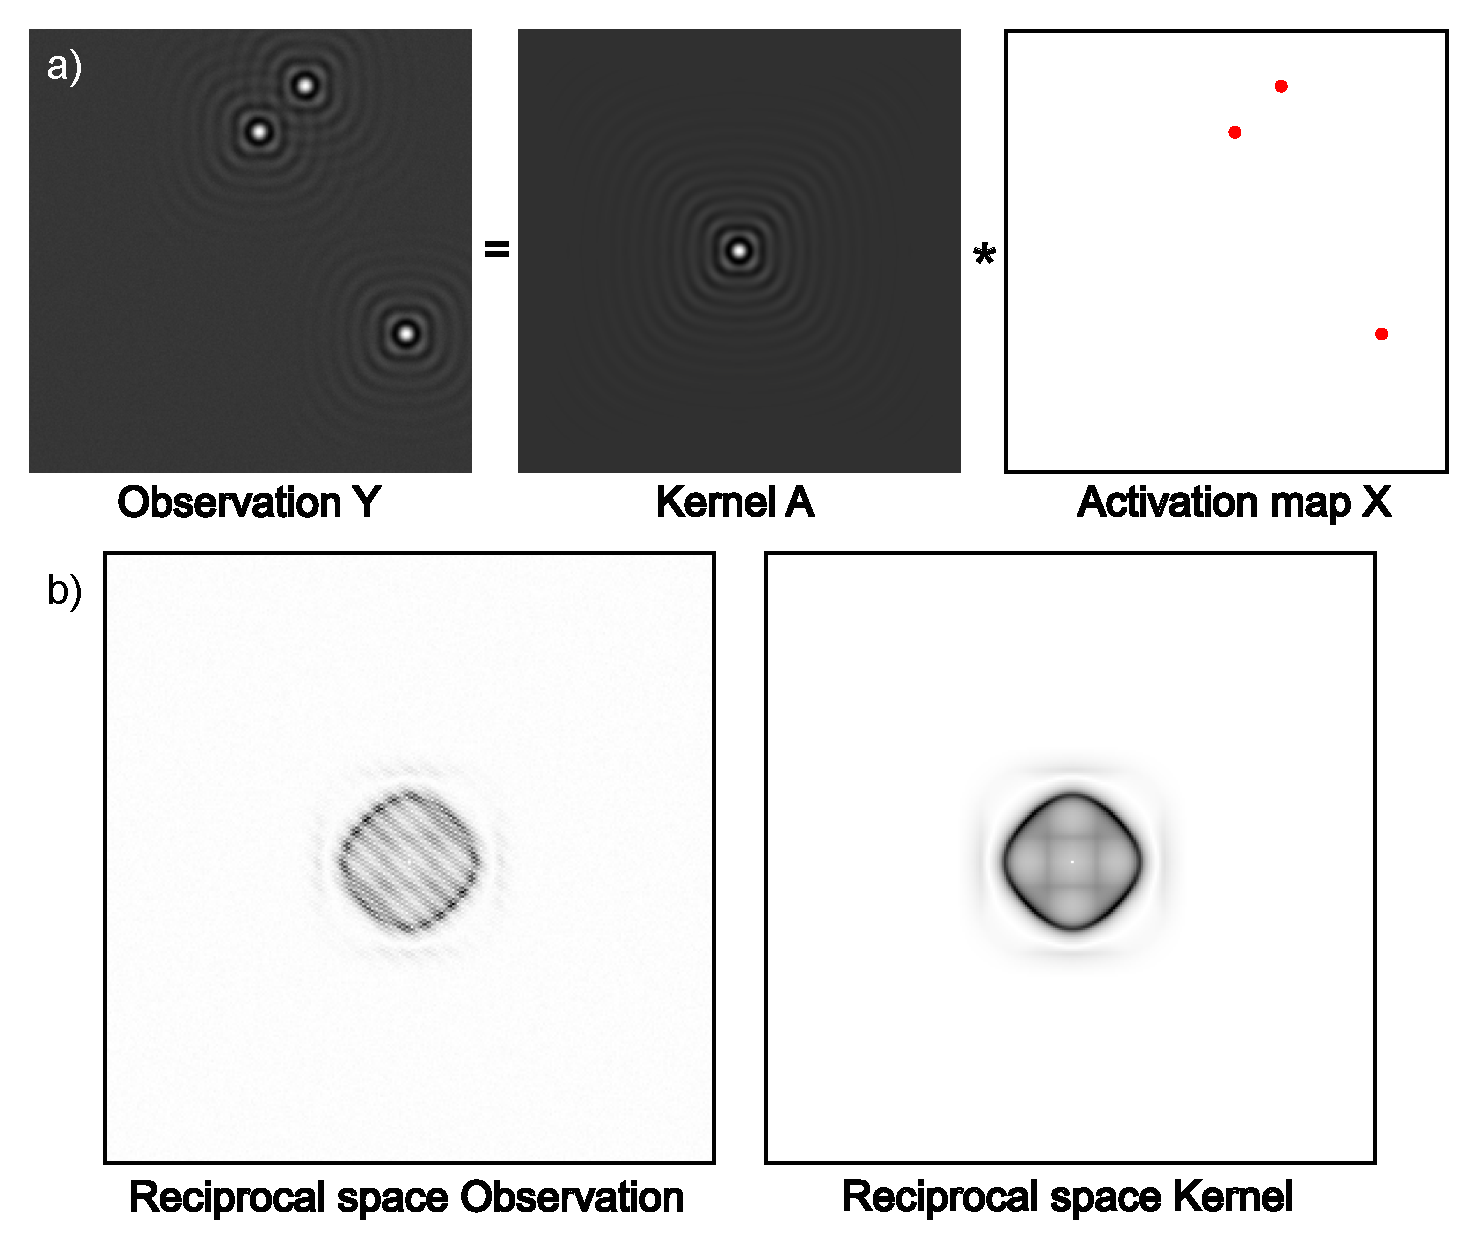
\includegraphics[width= \textwidth]{Ch6_deconvolution.pdf} 
	\centering
	\caption{}
	\label{fig:ch6_decon}
\end{figure}

\subsection{Demixing problem}
%todo: how should I include the general motivation of demxing? or is it enough here? 
Materials normally exhibit multiple types of defects, and these defects can present different scattering features; Many QPI measurements have exploited the mechanisms of selectivity scattering channels across a wide variety of materials, such as the sign variation of the superconducting order parameter, the spin and orbital texture of topological bands, etc. To study the mechanisms of these selection rules, we need to acquire \ac{QPI} patterns from individual types of defect; This can be achieved by finding isolated defects and taking grid maps on that. However, as mentioned in chapter 5, isolated defects are hard to find experimentally, it is even more difficult if we wish to obtain QPI measurements with high q-space resolution, as that requires a wider real space range. It is therefore preferred, if we can reconstruct the contribution of each individual type of defect from a big grid map that includes multiple types of defects; this is called the demixing problem.  

We now use our synthetic data to better illustrate the demixing problem. We simulate 2 \ac{QPI} patterns from 2 distinct defects with kernel choices A1 and A2 as shown in Fig. \ref{fig:ch6_demix} c) and d); We then define their activation maps X1 and X2 in d) and g). By summing up the convolutions between 2 kernels and their corresponding activation maps, we can obtain an observation Y in a). We express the above observation generation process as:
\begin{equation}
	Y = A1 * X1 + A2 * X2 + \beta, 
\end{equation}
where $\beta$ is the added noise determined by a pre-defined signal-to-noise ratio.

The demixing problem is the inverse of the observation generation process: given the observation 
Y, our goal is to reconstruct A1, A2, and their corresponding activation maps. This means that in reciprocal space, rather than working with entangled and less informative data like (b), we can recover disentangled QPI patterns from individual defect types, as shown in (e) and (h), which are also free from speckles. Lastly, we extend the above formulation with t types of different defects, then at arbitrary energy $\omega$, we have: 

\begin{equation}
	Y_{\omega} = \sum_T ( A_{T,{\omega}} * X_T) + \beta. 
\end{equation} 



\begin{figure}
	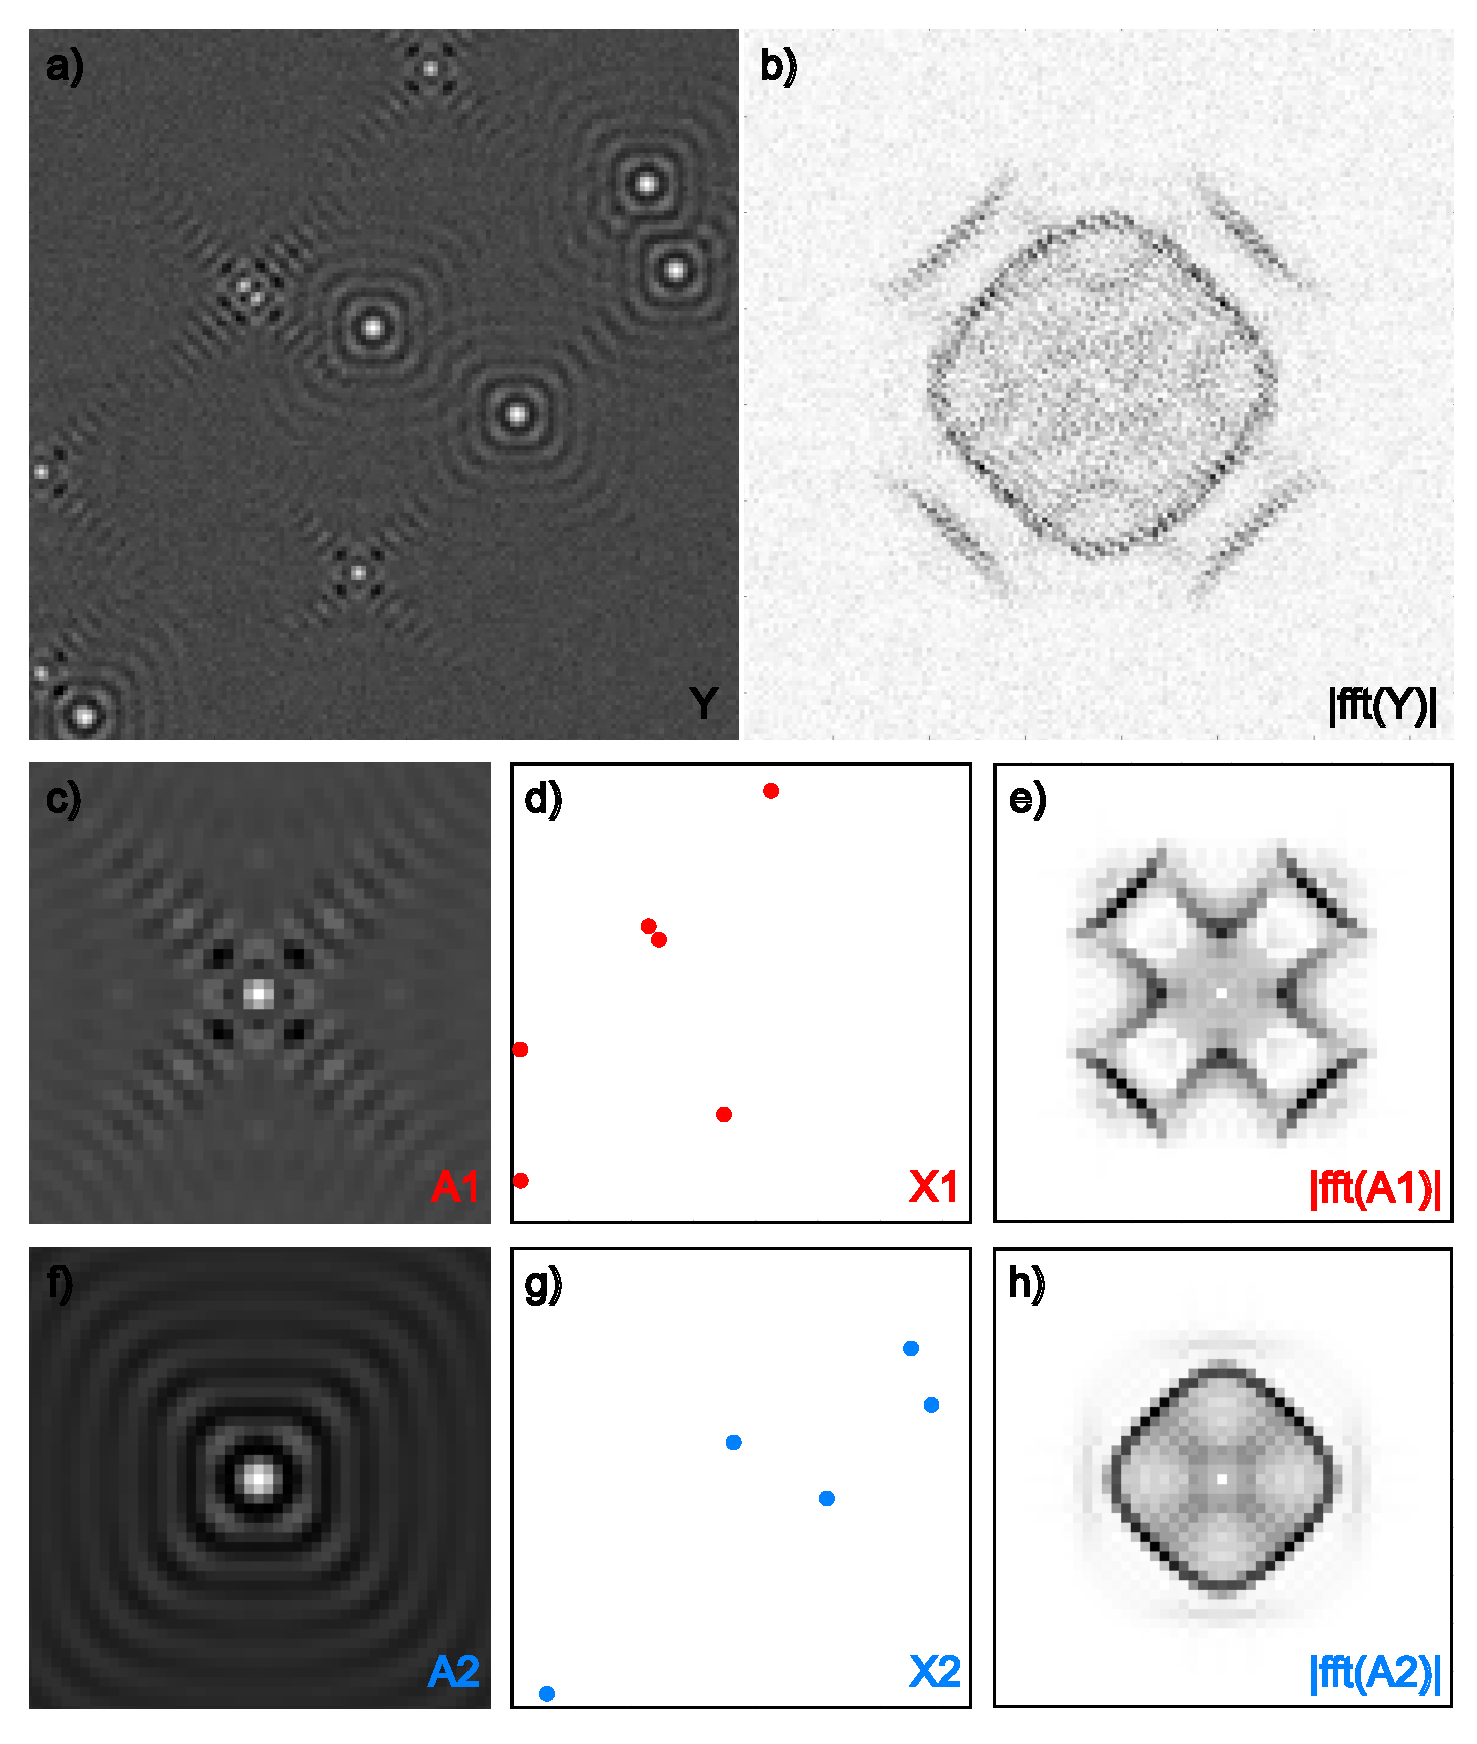
\includegraphics[width= \textwidth]{Ch6_demixing.pdf} 
	\centering
	\caption{}
	\label{fig:ch6_demix}
\end{figure}